\documentclass[a4paper, 11pt, oneside]{scrartcl}
\usepackage{lpp}
\usepackage{graphicx}
\usepackage{tikz}
\usetikzlibrary{shapes.geometric, arrows}

\begin{document}

\mtitle{Computer Science Report}

\mauthor{Mohsin Ali Chaudry, Raghavan Lakshmanan}{Abhishek Y. Deshmukh}

\maff{SiSc Laboratory}{W S}{2013/14}

%\mabstract{This engineering project of SiSc Lab involves the development of a parallel finite element
%solver using unstructured grids. The developed and optimized code is validated using
%analytical solutions for a time-dependent engineering heat
%transfer problem. This report consists of the approach followed for parallelizing the serial code.
%}

\section*{Task 1: Software engineering}
\textbf{a) Identify software process activities relevant to your project. Motivate your choices.}

The software process activities relevant to our project are described as follows:

\subsection*{Requirements Engineering:}
A software is developed that is able to solve numerically the heat diffusion equation to determine the temperature distribution either transient or steady state in a given domain of a physical problem using finite element approach on unstructured meshes.The software should deliver solution fast and should be able to handle large problem sizes. It should scale close to linear so that it can exploit high degree of parallelism.
\subsection*{Design and Implementation}
The software is implemented in C++ using Object Oriented approach. The software is structured in a modular way, each module representing a functionality such as mesh, solver, postprocessing, etc.
\subsection*{Verification}
The software has been verified against the analytical solutions of standard problems that are available in the literature.
%\subsection*{Evolution}
%The software has evolved according to the needs of customer from solving basic problems to more realistic physical applications.
\\
\\
\textbf{b) Identify models and techniques used. Motivate why these models and techniques were chosen.}

A Waterfall model is used as a software process model. This model is chosen because it has distinct phases of software activities described in last section. In this project, the requirements of the customer were well understood and they were not going to change over the development time. Also, it was easier to monitor the progress of the project through documentation at the end of each phase. 

Finite element modelling was chosen because it can deal with unstructured meshes which are useful in case complex physical domains. Keeping in the mind the future use of the results obtained through the software that could be used in structural analysis, finite element technique is the obvious choice. The implementation 

Object oriented approach was chosen as it enables to divide the code based on functionality and make it extendable and reusable for future expansion.

\section*{Task 2: Code organization}
\textbf{a) Describe the software versioning and revision control system used in your project. What features did you use? What features beyond those presented in the lecture do you find useful? Why?}

We have used SVN as the software versioning and revision control system in our project. A software repository with version control system is installed on a dedicated (central, accessible) server. It allows to control the access to the users specified by the administrator. It keeps track of all updates/changes. It allows to store additional information with each update of the sources. It allows to retrieve older versions of the code. It is flexible to grow with the code and/or group of developers, allows to set up "branches" from the main repository. It also provides an information distribution system (e.g. mail to a list at each "commit" event). The basic idea is get rid of the private/local copies. 

We used following commands:

- svn co <address> (Check out the repository)

- svn up (Update the current repository)

- svn add (Add files/folders to the repository)

- svn delete (Delete unnecessary files/folders)

- svn commit -m"Message" (Commit the changes)

In addition to these commands, we also used following command which was useful in creating a copy for branching out to parallel code.

- svn cp <directory>
\\
\textbf{b) How do you ensure the portability of your code? How do you ensure any user can install and run your code?}

In general, C++ is a portable language. At the most, the user will have to recompile the code using makefile to link the VTK libraries. We have used standard C++ constructs. The code can be compiled with both gnu and intel compilers on most of the machines. There are no special machine/architecture specific constructions.
\\
\\
\textbf{c) Identify parts of your code which could be placed in a separate library. Motivate your choice.}

Our code is divided based on functionality such as input settings, mesh processing, solver and visualization. These can be placed in separate libraries which can be reusable in other codes. Post processing is based on VTK library. However, input settings are specific to the code. Mesh and solver parts can be safely placed in separate libraries as they are independent. 
\\
\\
\textbf{d) Explain and motivate the style for commeting used in your code.}

The style of commenting is chosen so as to be compatible with Doxygen. Doxygen generates the code documentation automatically based on the comments in the source code. It also generates call graphs which are useful in understanding overall structure of the software. Multiline comments are enclosed between "/*!<comments>*/" while single liners can be preceded by "/// <comment>". Doxygen identifies these comments and generates an online-browser documentation or LATEX document based on the options provided in Doxyfile.

\section*{Task 3: Testing and debugging}
\textbf{a) Describe the debugging systems(s) you used for developing your application.}

Following debugging systems were used in developing the application:

\textbf{1. "Printf" debugging:} Printing the considered variables in the output stream and checking if they have expected values. This is the easiest form of debugging but can take time to identify the bugs in the code. We used it extensively.

\textbf{2. gdb:} This is a useful tool for debugging of serial code whenever segmentation fault occurs. The backtrace can be anaylsed to identify where the code is trying to access the value at an undesired location. We used it when  "Printf debugging" failed to identify the bug.

\textbf{3. Totalview:} This is a multiprocess and multithread debugging tool. This is used in debugging parallel version of our code.
\\
\\
\textbf{b) How do you ensure that the code you have created is correct? What kind of tests did you run?}

The correctness of code was ensured by testing the code at each stage and making sure each of the submodule is working correctly. We tested the individual parts of the code for the expected output. If the individual parts are correct then overall program should give correct output. Finally full code was validated against the analytical solutions available in literature. We also applied some tests which check that the solution is not unphysical. e.g. The temperature (in Kelvin) should not be negative.

In terms of the correctness of the software constructs, the MPI standard was followed while writing the parallel code.
\\
\\
\textbf{c) Which of the testing techniques presented (or others, if applicable) did you employ? Why?}

We employed following testing techniques:

\textbf{1. Color Box testing:}
Color box testing includes white box, black box and grey box testing. All of these testing techniques were applied at some stage of development of the code. Grey box testing was used extensively to check the working of individual units. White box testing was used in developing postprocessing module where it has to be linked to VTK library. Finally black box testing in validating the code, whether the code does what it is supposed to do. 

\textbf{2. Sanity testing:}
Sanity testing was used to identify the unusual problems which are difficult to identify. e.g. If the temperature in the domain is initialized to 300 K and all boundaries are at 300 K, over the time, the temperature should not change. This helped to identify a bug in the solver part.

\textbf{3. Performance testing:}
Performance testing was done to identify where the code can be tuned to improve.

\textbf{4. Scalability testing:} 
Scalability testing is to check if the parallel version of the code is able to harness the parallelism from the available architecture. It showed that our code is able to achieve reasonable scaling though there is still scope to improve it.
\\
\\
\textbf{d) Did you have structured approach to testing when devloping your application? If you did, are there any advantages that you have observed to having a structured approach to testing? If not, what are the advantages of the unstructured approach? Why?}

Yes, we had a structured approach while developing the application. We made sure that individual components of the application work and they work correctly. The serial code was first validated with smaller structured mesh before moving to bigger unstructured meshes. Testing with smaller meshes helped us in manually checking the output for expected values. While testing if a bug was found, this structured approach helped to focus on the module where the problem is. This is similar to divide and conquer approach.
\section*{Task 4: Performance}
\textbf{a) What tools and techniques have you used to ensure the performance of you code? Why?}

The performance of the code was improved by manual optimization and scalar optimization tools provided by compiler. The scalar optimization includes manually changing the code to exploit spatial and temporal locality by measures such as loop unrolling, storing reused variables as local so as to avoid cache misses, etc. There are automatic compiler optimization options such as O1, O2 and O3. We have done manual optimization wherever possible as described above and on the top of that, the highest level of automatic optimization, O3, is employed to ensure maximum performance while keeping good machine accuracy. To improve parallel performance, we used "Scalasca" to find the inefficiencies in the code and tried to improve them.
\\
\\
\textbf{b) Describe the performance improvements you have obtained by tuning your code.}

Following table (also fig. 1) shows the performance improvements obtained by scalar optimization:

\begin{tabular}{|c|c|c|}
\hline 
Optimization Level & Time (s) & Speedup \\ 
\hline 
O0 & 3.62E+001 & 1 \\ 
\hline 
O1 & 7.97E+000 & 4.542 \\ 
\hline 
O2 & 7.79E+000 & 4.647 \\ 
\hline 
O3 & 6.45E+000 & 5.612 \\ 
\hline 
\end{tabular} 
\\
\\
Compiler optimization has made the code 5.6 times faster. The manual optimization was already followed while writing the code so there is no unoptimized code available to measure the performance of manual optimization against it.
\\
\\
\textbf{c) Describe further ways you could improve performance if you had more time.}

If we had more time, we could have tried to come up with different strategies to parallelize the code to improve the scaling. We already tried three different strategies. All three have some advantages and some disadvantages. We could have tried to combine the two approaches of parallelizing to see if we can get the advantages of both and do away with the drawbacks. In one approach, we are communicating the boundary data in round-robin fashion using two-sided communication. This approach performed the worst. In second approach, we are communicating node to node information on the boundaries. This increases communication overhead. In third approach, we tried to use one-sided communication, but node to node communication on boundaries. The scalability is shown in fig. 2.

\begin{figure}[!htb]
\centering
\minipage{0.5\textwidth}
\centering
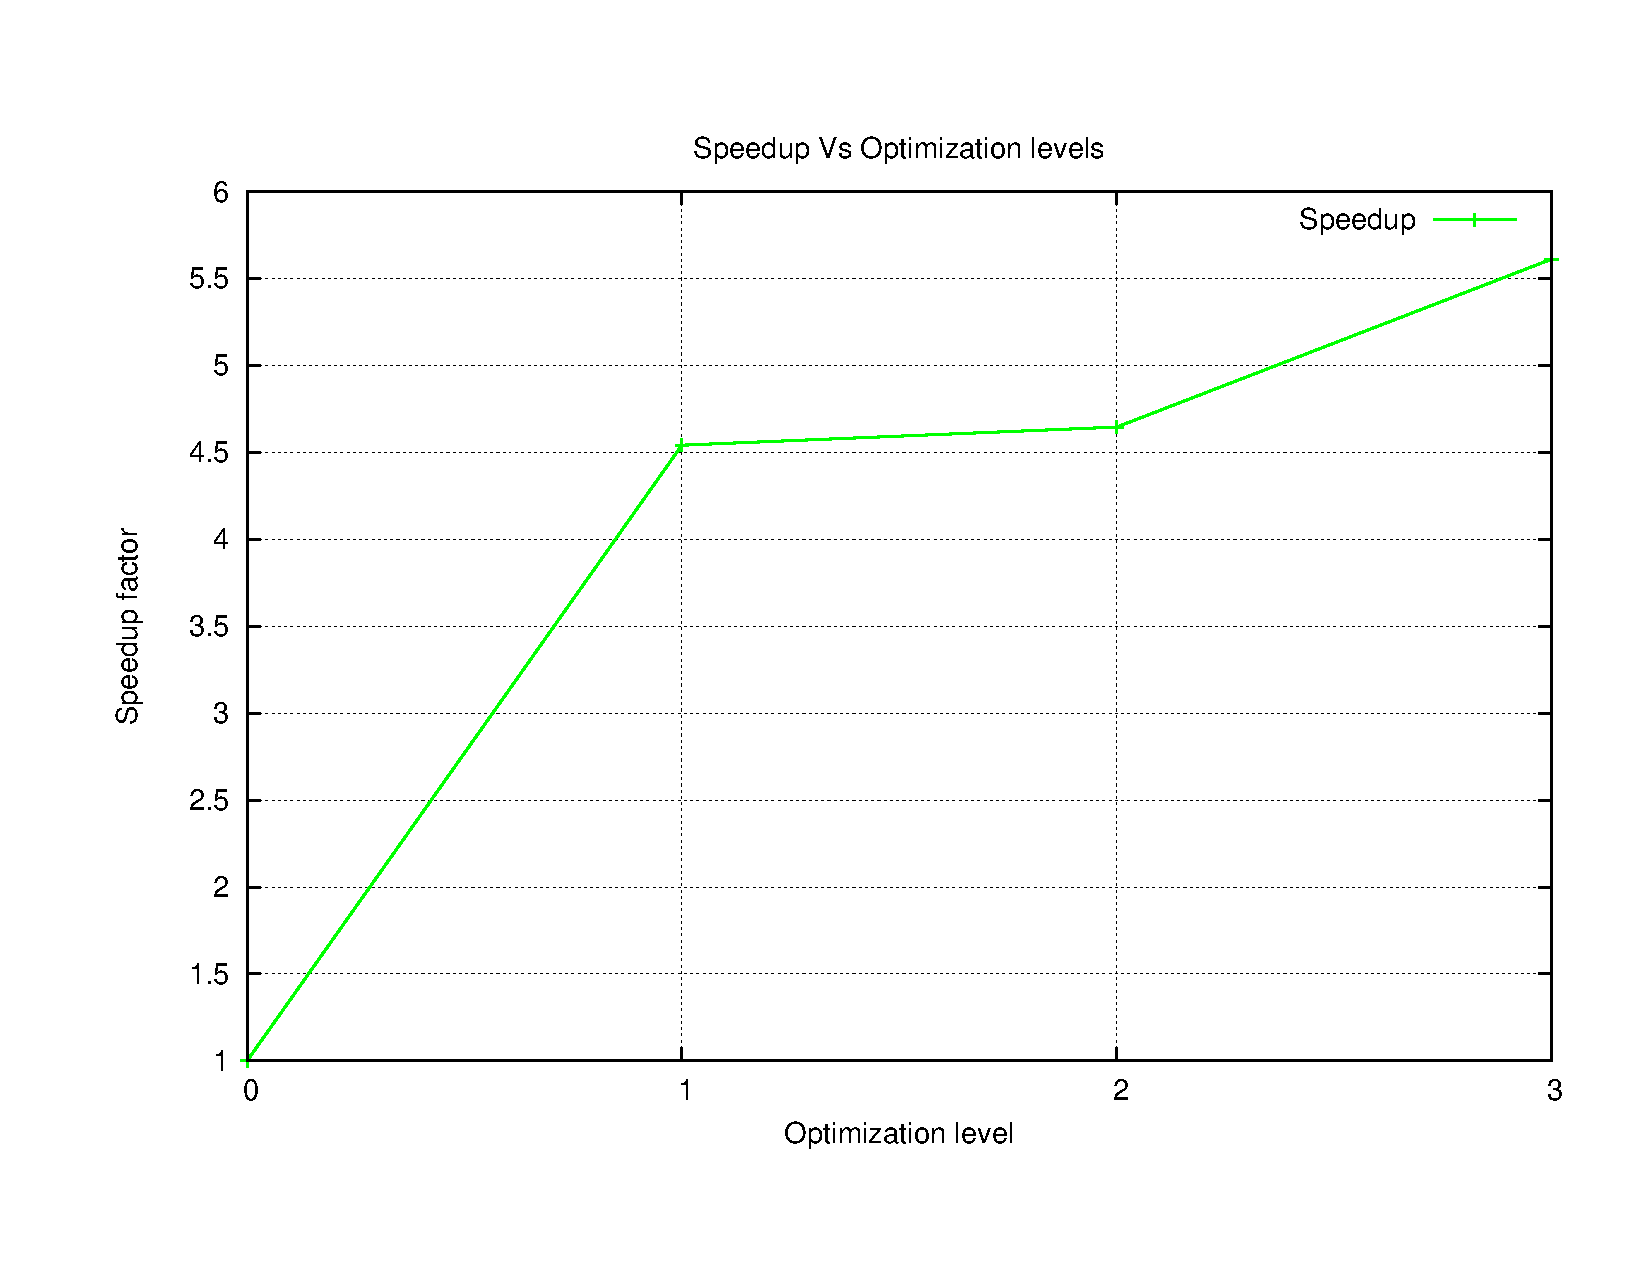
\includegraphics[scale=0.33]{./Performance.pdf}
\caption{Scalar Optimization}
\endminipage\hfill
\centering
\minipage{0.5\textwidth}
\centering
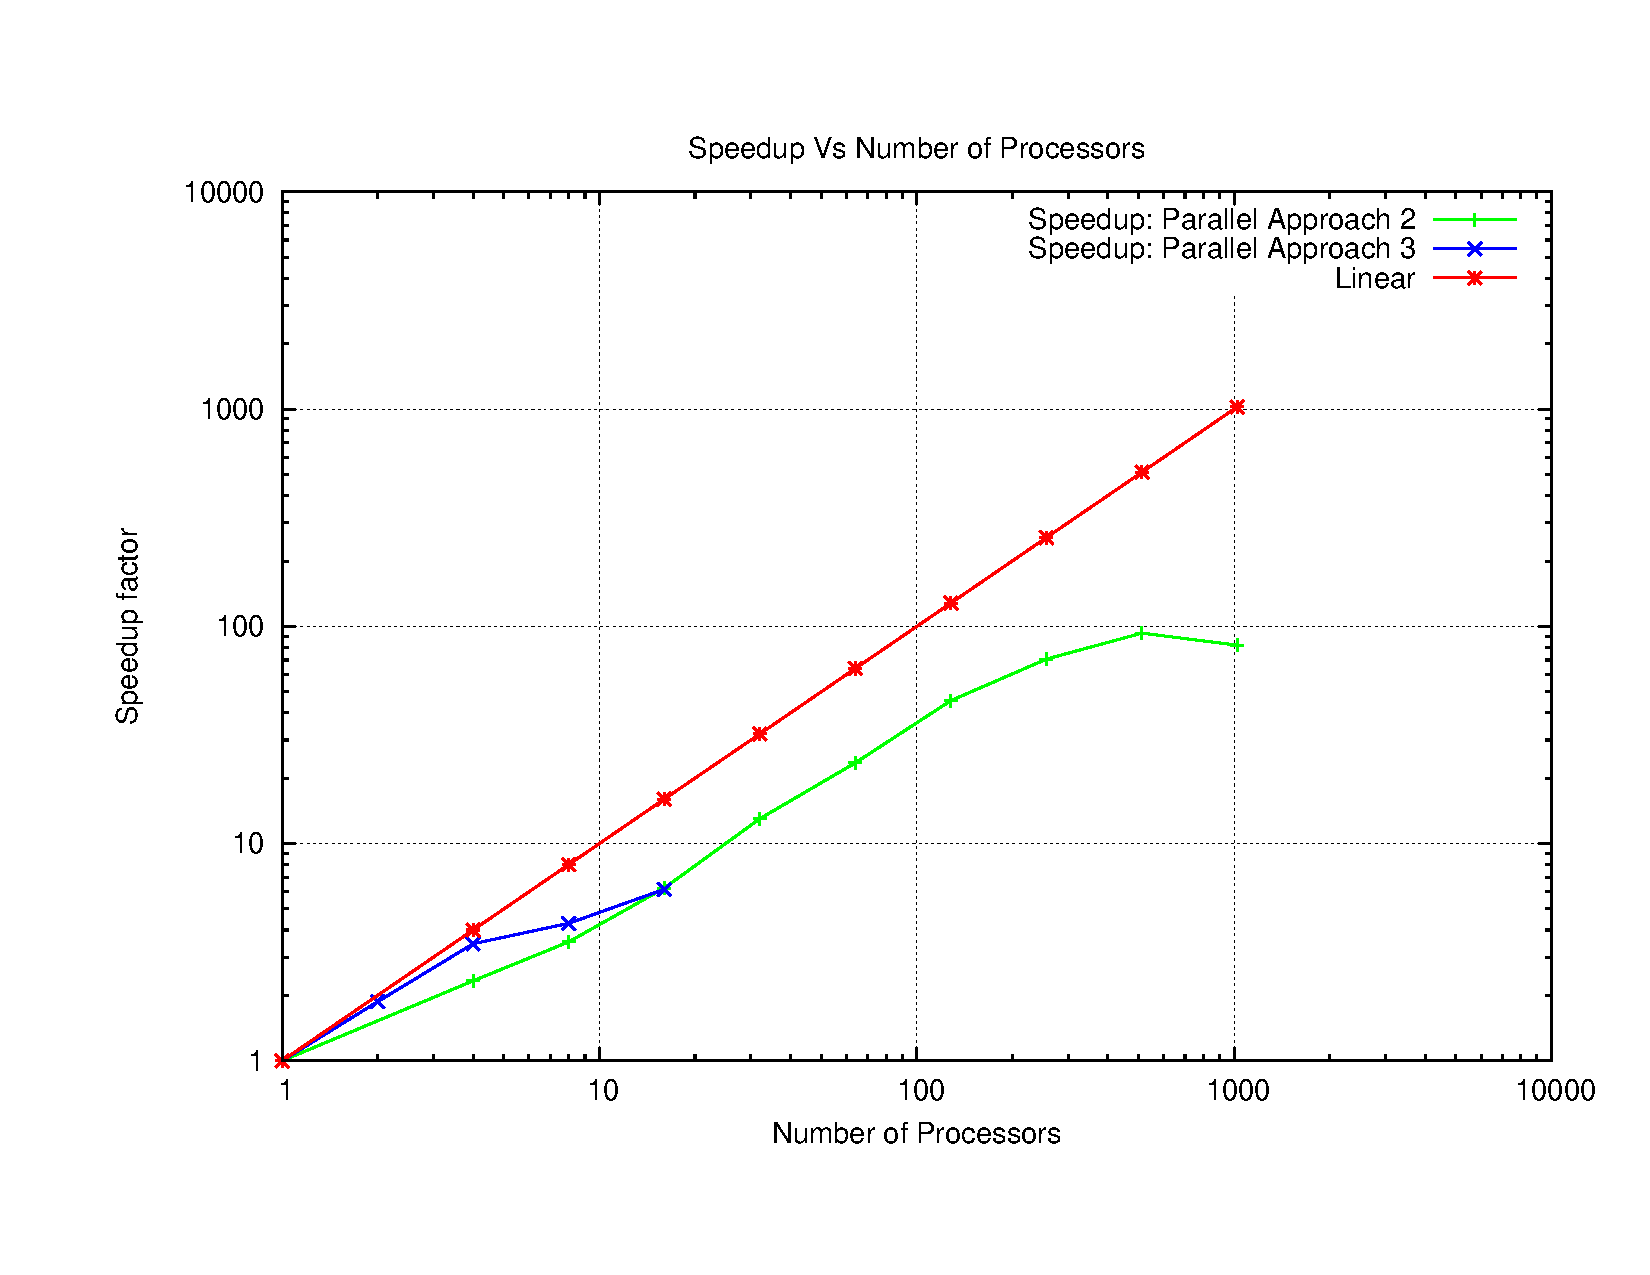
\includegraphics[scale=0.33]{./parallel.pdf}
\caption{Scalability}
\endminipage\hfill
\end{figure}


\end{document}
